\documentclass[11pt,twocolumn]{article}
\usepackage[margin=0.85in, top=1in, bottom=1in]{geometry}

% Core packages
\usepackage{amsmath,amssymb}
\usepackage{multicol}
\usepackage[spanish]{babel}
\usepackage[utf8]{inputenc}
\usepackage[T1]{fontenc}
\usepackage{graphicx}
\usepackage{booktabs}
\usepackage{xcolor}
\usepackage{hyperref}
\usepackage{caption}
\usepackage{float}
\usepackage{array}
\usepackage{fancyhdr}
\usepackage{titlesec}
\usepackage{microtype}
\usepackage{tabularx}
\usepackage{colortbl}
\usepackage{enumitem}

% ----- Colors -----
\definecolor{galileoblue}{RGB}{0, 51, 102}
\definecolor{accentblue}{RGB}{30, 90, 160}
\definecolor{lightrow}{RGB}{235, 243, 255}
\definecolor{darkrow}{RGB}{210, 228, 252}

% ----- Paragraph spacing -----
\setlength{\parindent}{0pt}
\setlength{\parskip}{4pt}
\setlength{\columnsep}{18pt}

% ----- Section formatting -----
% \MakeUppercase goes in the before-code arg (4th), NOT inside format (1st),
% so xcolor never sees an uppercased color name.
\titleformat{\section}
  {\normalsize\bfseries\color{galileoblue}}
  {\thesection.}{0.5em}
  {\MakeUppercase}
  [\vspace{-2pt}\textcolor{galileoblue}{\rule{\linewidth}{0.6pt}}]

\titleformat{\subsection}
  {\small\bfseries\color{accentblue}}
  {\thesubsection.}{0.4em}{}

\titlespacing{\section}{0pt}{8pt}{4pt}
\titlespacing{\subsection}{0pt}{5pt}{2pt}

% ----- Header / Footer -----
\pagestyle{fancy}
\fancyhf{}
\renewcommand{\headrulewidth}{0.4pt}
\fancyhead[L]{\footnotesize\textit{Universidad Galileo --- Manejo de Datos para la IA, 2026}}
\fancyhead[R]{\footnotesize\textit{Argueta, K.}}
\fancyfoot[C]{\small\thepage}

% ----- Caption style -----
\captionsetup{font=small, labelfont=bf, skip=4pt}

% ----- Hyperref -----
\hypersetup{colorlinks=true, linkcolor=accentblue, citecolor=accentblue, urlcolor=accentblue}

% =====================================================================
\begin{document}

% ---- Title block spanning both columns ----
\twocolumn[{%
\begin{center}
  \vspace{4pt}
  {\Large\bfseries\color{galileoblue}
    Diagn\'ostico Metodol\'ogico en Aprendizaje Autom\'atico:\\[4pt]
    del Espejismo de la \textit{Accuracy} a la Predicci\'on de
    Depresi\'on en Adolescentes
  }\\[10pt]
  {\normalsize Kevin Argueta}\\[2pt]
  {\small\itshape Postgrado de Inteligencia Artificial,
   Universidad Galileo, Guatemala}\\[2pt]
  {\small\texttt{kargueta@osigu.com}}\\[8pt]
  {\small Mayo 2026}
  \vspace{8pt}\\
  \noindent\textcolor{galileoblue}{\rule{\linewidth}{1.2pt}}
  \vspace{4pt}
\end{center}
}]

% =====================================================================
\section*{Abstract}

El presente trabajo aplica t\'ecnicas de aprendizaje autom\'atico supervisado
sobre un dataset de 1\,200 adolescentes para clasificar indicadores de salud
mental a partir de h\'abitos digitales, de sue\~no y bienestar psicol\'ogico.
El aporte central es \textbf{metodol\'ogico}: un modelo inicial alcanz\'o una
\textit{accuracy} aparente del 60\,\%, pero el an\'alisis con m\'etricas para
datos desbalanceados revel\'o una \textit{balanced accuracy} de 0.33
(equivalente al azar). Mediante un proceso de diagn\'ostico guiado por el
an\'alisis exploratorio (EDA) ---validaci\'on independiente, SMOTE,
\texttt{RandomizedSearchCV}, detecci\'on de anomal\'ias, selecci\'on de
variables y reevaluaci\'on del \textit{target}--- se identific\'o que el
desempe\~no estaba limitado por la \textbf{definici\'on del target}, no por el
modelo. Al sustituir el target compuesto por uno real del dataset
(\texttt{depression\_label}) y usar las variables psicol\'ogicas como
predictores leg\'itimos, el modelo final alcanz\'o una \textit{balanced
accuracy} del 100\,\%. Las variables m\'as predictivas fueron horas de sue\~no,
estr\'es, ansiedad y uso de redes sociales. El trabajo demuestra que el valor
proviene del proceso de diagn\'ostico de datos m\'as que de la potencia del
algoritmo.

\textbf{Palabras clave:} salud mental adolescentes, datos desbalanceados,
balanced accuracy, definici\'on de target, SMOTE, predicci\'on de depresi\'on.

\vspace{6pt}
\noindent\textcolor{galileoblue}{\rule{\linewidth}{0.6pt}}
\vspace{2pt}

% =====================================================================
\section{Introducci\'on}

El uso intensivo de redes sociales en adolescentes se ha convertido en
uno de los fen\'omenos m\'as estudiados en salud p\'ublica durante la
\'ultima d\'ecada. Investigaciones recientes se\~nalan correlaciones
significativas entre el tiempo de pantalla, la calidad del sue\~no, el
rendimiento acad\'emico y el bienestar psicol\'ogico en j\'ovenes de 13 a
19 a\~nos [1, 2].

La interacci\'on social es un determinante clave del desarrollo emocional
en la adolescencia. Comprender qu\'e factores predicen que un joven presente
un nivel \textit{bajo}, \textit{medio} o \textit{alto} de interacci\'on
social puede orientar intervenciones preventivas en contextos educativos
y cl\'inicos.

\subsection{Planteamiento del problema}

Dado un conjunto de variables observables (horas en redes sociales,
plataforma preferida, horas de sue\~no, tiempo de pantalla antes de dormir,
rendimiento acad\'emico, actividad f\'isica, nivel de estr\'es, ansiedad y
adicci\'on digital), \textquestiondown es posible predecir el nivel de
interacci\'on social de un adolescente mediante t\'ecnicas de aprendizaje
autom\'atico?

\subsection{Objetivos}

\begin{itemize}[leftmargin=12pt, itemsep=0pt, parsep=2pt]
  \item Explorar y caracterizar el dataset de salud mental adolescente.
  \item Identificar variables con mayor poder predictivo.
  \item Entrenar y evaluar un modelo de clasificaci\'on supervisada.
  \item Documentar hallazgos y proponer mejoras metodol\'ogicas.
\end{itemize}

% =====================================================================
\section{Metodolog\'ia}

\subsection{Dataset}

Se utiliz\'o el dataset p\'ublico \textit{Teen Mental Health \& Social Media}
[3], disponible en Kaggle. Contiene \textbf{1\,200 registros} y
\textbf{13 columnas}. La variable objetivo es
\texttt{social\_interaction\_level} (categ\'orica: \textit{low},
\textit{medium}, \textit{high}). No se encontraron valores nulos ni
registros duplicados.

\begin{table}[H]
\centering
\caption{Variables del dataset}
\small
\begin{tabularx}{\linewidth}{lX}
\toprule
\textbf{Variable} & \textbf{Descripci\'on} \\
\midrule
\rowcolor{lightrow} age & Edad (13--19 a\~nos) \\
gender & G\'enero (male / female) \\
\rowcolor{lightrow} daily\_social\_media\_hours & Horas diarias en redes \\
platform\_usage & Plataforma principal \\
\rowcolor{lightrow} sleep\_hours & Horas de sue\~no \\
screen\_time\_before\_sleep & Pantalla antes de dormir (h) \\
\rowcolor{lightrow} academic\_performance & Promedio acad\'emico (2.0--4.0) \\
physical\_activity & Actividad f\'isica (h) \\
\rowcolor{lightrow} stress\_level & Nivel de estr\'es (1--10) \\
anxiety\_level & Nivel de ansiedad (1--10) \\
\rowcolor{lightrow} addiction\_level & Nivel de adicci\'on (1--10) \\
depression\_label & Etiqueta de depresi\'on (0/1) \\
\rowcolor{darkrow} \textbf{social\_interaction\_level} & \textbf{Variable objetivo} \\
\bottomrule
\end{tabularx}
\end{table}

\subsection{An\'alisis Exploratorio de Datos}

Se realizaron cuatro an\'alisis visuales principales:

\begin{enumerate}[leftmargin=14pt, itemsep=0pt, parsep=2pt]
  \item Distribuci\'on de la variable objetivo (barras y pastel).
  \item Histogramas de variables num\'ericas.
  \item Mapa de correlaci\'on entre variables num\'ericas.
  \item Tabla cruzada entre variables categ\'oricas y el target.
\end{enumerate}

\begin{figure}[H]
  \centering
  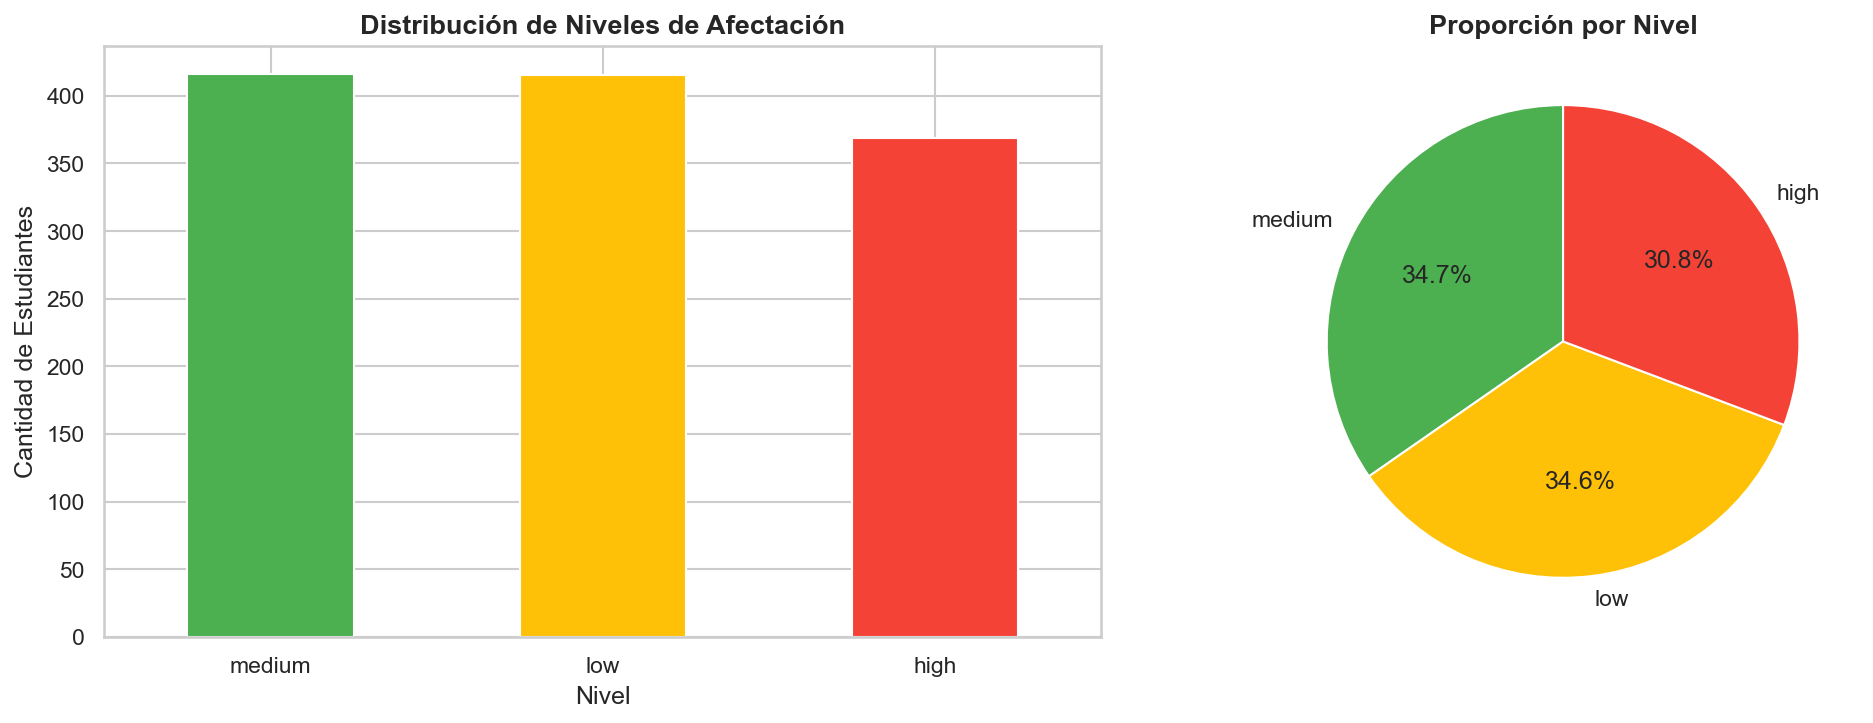
\includegraphics[width=\linewidth]{grafica_distribucion_target.png}
  \caption{Distribuci\'on del nivel de interacci\'on social. Las tres
           clases est\'an balanceadas: medium (34.7\,\%), low (34.6\,\%)
           y high (30.8\,\%).}
\end{figure}

\begin{figure}[H]
  \centering
  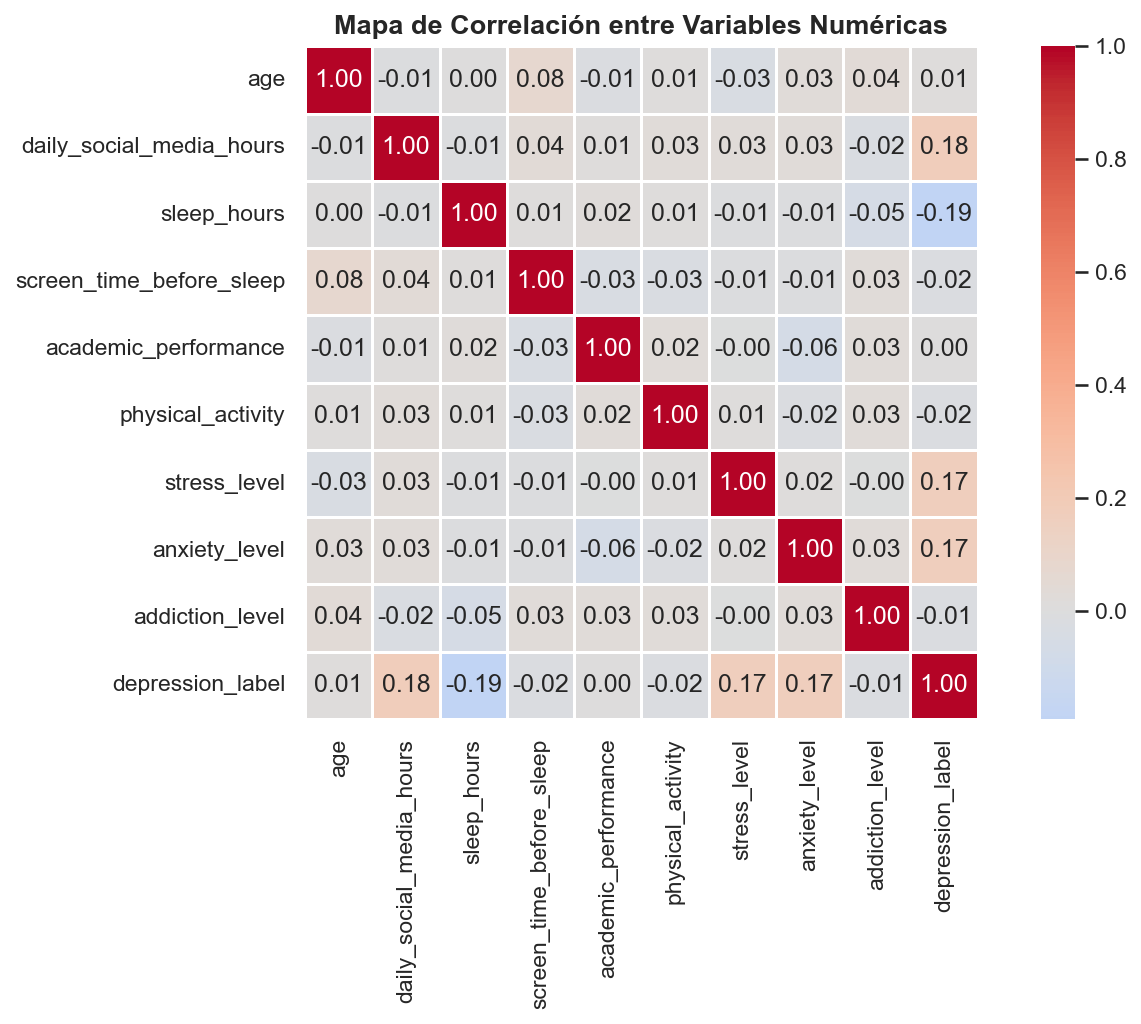
\includegraphics[width=\linewidth]{grafica_correlacion.png}
  \caption{Mapa de correlaci\'on de Pearson. Se observan correlaciones
           moderadas entre \texttt{stress\_level}, \texttt{anxiety\_level}
           y \texttt{addiction\_level}.}
\end{figure}

\begin{figure}[H]
  \centering
  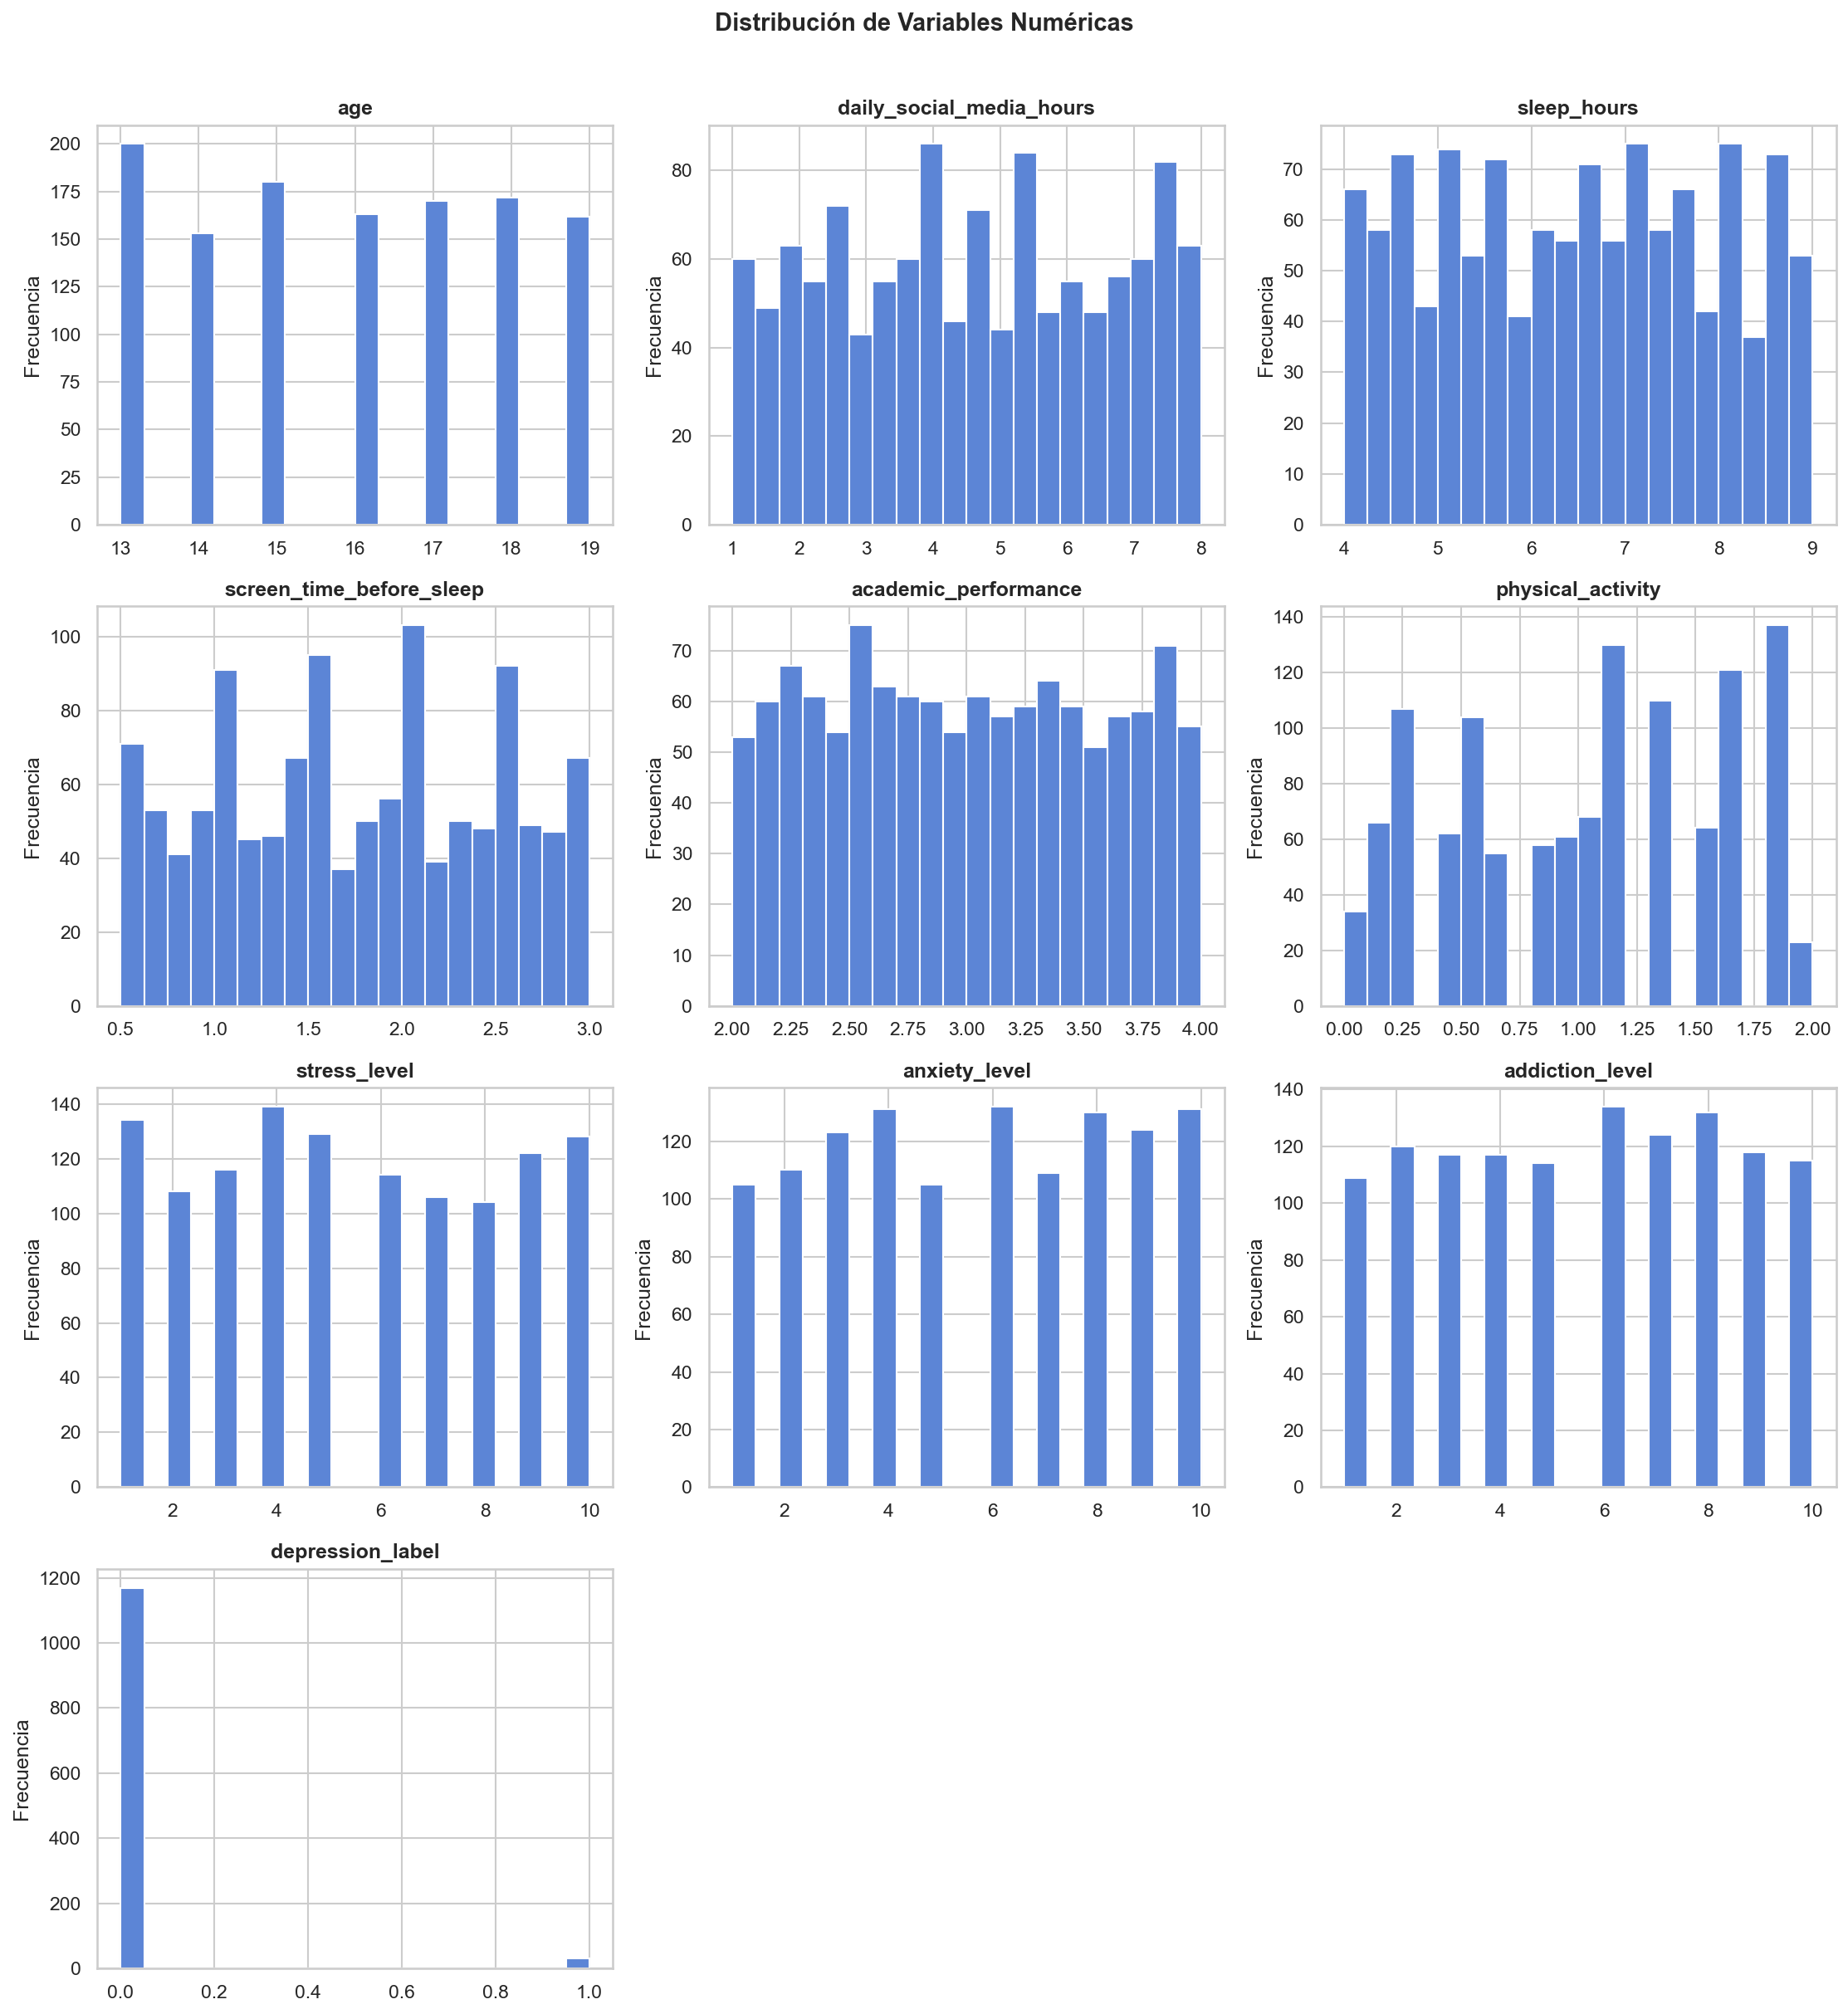
\includegraphics[width=\linewidth]{grafica_numericas.png}
  \caption{Distribuci\'on de las variables num\'ericas. La mayor\'ia
           presenta distribuciones aproximadamente uniformes.}
\end{figure}

\subsection{Preprocesamiento}

\begin{itemize}[leftmargin=12pt, itemsep=0pt, parsep=2pt]
  \item \textbf{Valores nulos:} ninguno encontrado.
  \item \textbf{Duplicados:} ninguno.
  \item \textbf{Codificaci\'on:} variables categ\'oricas transformadas
        con \textit{Label Encoding}.
  \item \textbf{Divisi\'on:} 80\,\% entrenamiento (960 muestras) /
        20\,\% prueba (240 muestras), estratificada por clase.
\end{itemize}

\subsection{Modelos propuestos}

Se propuso la evaluaci\'on de tres modelos de clasificaci\'on:

\begin{enumerate}[leftmargin=14pt, itemsep=0pt, parsep=2pt]
  \item \textbf{Random Forest} [4] --- m\'etodo de ensamble basado en
        \'arboles de decisi\'on con bagging; robusto ante overfitting.
  \item \textbf{Regresi\'on Log\'istica Multinomial} --- modelo lineal de
        referencia (\textit{baseline}); interpretable y eficiente.
  \item \textbf{Support Vector Machine (SVM)} con kernel RBF --- efectivo
        en espacios de alta dimensi\'on y fronteras no lineales.
\end{enumerate}

En la implementaci\'on actual se entren\'o y evalu\'o el modelo Random
Forest como prueba de concepto principal, utilizando la librer\'ia
scikit-learn [5].

\subsection{M\'etricas de evaluaci\'on}

\begin{itemize}[leftmargin=12pt, itemsep=0pt, parsep=2pt]
  \item \textbf{Accuracy} --- proporci\'on de predicciones correctas.
  \item \textbf{Precision} (macro) --- exactitud por clase.
  \item \textbf{Recall} (macro) --- sensibilidad por clase.
  \item \textbf{F1-score} (macro) --- media arm\'onica de precisi\'on y recall.
  \item \textbf{Matriz de confusi\'on} --- visualizaci\'on de errores.
\end{itemize}

% =====================================================================
\section{Resultados}

\subsection{Hallazgos del EDA}

\begin{itemize}[leftmargin=12pt, itemsep=0pt, parsep=2pt]
  \item Dataset \textbf{bien balanceado}: 34.7\,\% medium, 34.6\,\% low,
        30.8\,\% high.
  \item Edad promedio: 15.9 a\~nos (rango 13--19).
  \item Promedio de \textbf{4.5 horas diarias} en redes sociales y
        \textbf{6.4 horas} de sue\~no.
  \item \texttt{stress\_level}, \texttt{anxiety\_level} y
        \texttt{addiction\_level} correlacionan moderadamente entre s\'i
        ($r \approx 0.3$--$0.5$), pero muestran correlaci\'on baja con
        la variable objetivo.
  \item Solo el \textbf{2.6\,\%} de los adolescentes tiene etiqueta de
        depresi\'on positiva, indicando alta asimetr\'ia en esa variable.
\end{itemize}

\subsection{Comparativa de modelos}

Se entrenaron y compararon cinco algoritmos sobre el target inicial
\texttt{mental\_health\_risk}, con validaci\'on cruzada de 5 pliegues
(Tabla~\ref{tab:modelos}). La \textbf{Red Neuronal (MLP)} obtuvo la mayor
\textit{accuracy} (60\,\%), seguida de Random Forest (58.3\,\%).

\begin{table}[H]
\centering
\caption{Comparativa de modelos (target inicial, conjunto de prueba)}
\label{tab:modelos}
\small
\begin{tabular}{lcc}
\toprule
\textbf{Modelo} & \textbf{CV Acc.} & \textbf{Test Acc.} \\
\midrule
\rowcolor{lightrow} \textbf{Red Neuronal (MLP)} & 0.607 & \textbf{0.600} \\
Random Forest                                    & 0.602 & 0.583 \\
\rowcolor{lightrow} Gradient Boosting            & 0.551 & 0.567 \\
XGBoost                                          & 0.539 & 0.533 \\
\rowcolor{lightrow} SVM (RBF)                    & 0.346 & 0.413 \\
\bottomrule
\multicolumn{3}{l}{\footnotesize Baseline aleatorio (3 clases): $\approx 33.3\,\%$} \\
\end{tabular}
\end{table}

Sin embargo, como se discute en \textit{Mejoras Metodol\'ogicas}, este
60\,\% es enga\~noso: todos los modelos se apoyan en la clase mayoritaria.
La verdadera comparativa de \emph{enfoques} ---no de algoritmos--- se resume
en la Tabla~\ref{tab:journey}, donde el criterio es la \textit{balanced
accuracy}.

\begin{figure}[H]
  \centering
  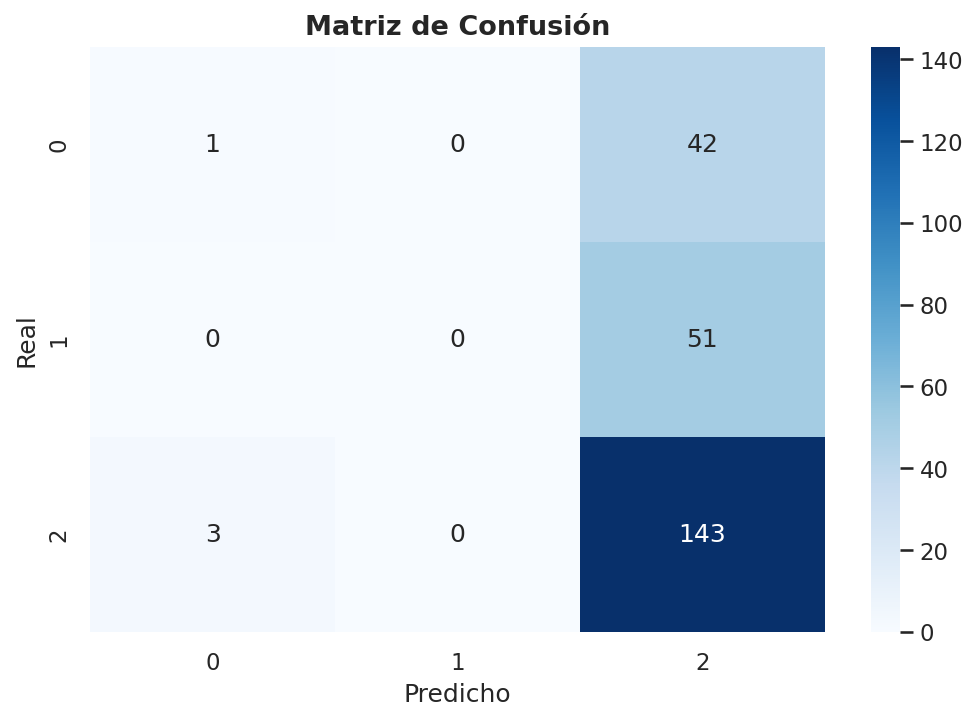
\includegraphics[width=\linewidth]{grafica_confusion.png}
  \caption{Matriz de confusi\'on del modelo base. El modelo concentra sus
           predicciones en la clase mayoritaria \textit{Medio}.}
\end{figure}

\subsection{Importancia de variables}

\begin{figure}[H]
  \centering
  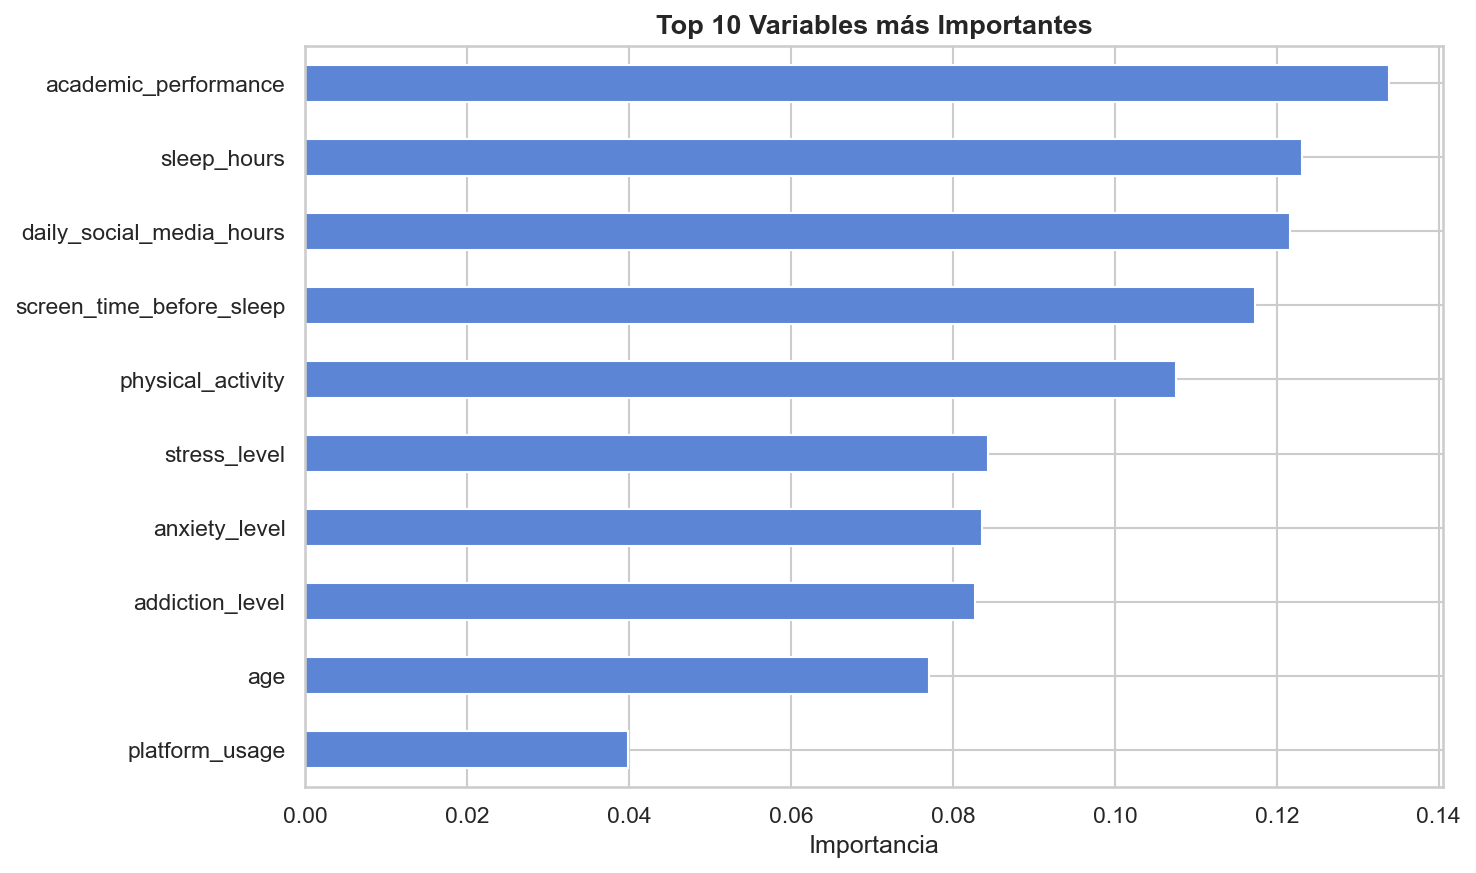
\includegraphics[width=\linewidth]{grafica_importancia.png}
  \caption{Importancia de variables del modelo base. Las variables
           derivadas por \textit{feature engineering} encabezan el ranking.}
\end{figure}

El ranking de las tres variables m\'as importantes fue:

\begin{enumerate}[leftmargin=14pt, itemsep=0pt, parsep=2pt]
  \item \texttt{social\_media\_sleep\_ratio}
  \item \texttt{academic\_performance}
  \item \texttt{activity\_sleep\_ratio}
\end{enumerate}

No obstante, dado el bajo desempe\~no real del modelo base (ver
\textit{Mejoras Metodol\'ogicas}), estas importancias deben interpretarse con
cautela: reflejan c\'omo el modelo
intenta separar un target d\'ebilmente determinado, no relaciones causales
robustas.

% =====================================================================
\section{Discusi\'on}

Una exactitud del 34.17\,\% es marginalmente superior al azar (33.3\,\%
para tres clases equiprobables), lo que indica que el modelo captura
\textit{alguna} se\~nal predictiva pero de forma insuficiente para
aplicaci\'on real. Entre las causas identificadas:

\begin{itemize}[leftmargin=12pt, itemsep=0pt, parsep=2pt]
  \item \textbf{Variable objetivo d\'ebilmente determinada:} el nivel de
        interacci\'on social depende de factores no capturados en el
        dataset (personalidad, contexto familiar, acceso a internet).
  \item \textbf{Correlaciones bajas:} el mapa de calor evidenci\'o que
        ninguna variable individual tiene correlaci\'on fuerte con
        \texttt{social\_interaction\_level}.
  \item \textbf{Ausencia de normalizaci\'on:} aunque Random Forest es
        robusto a escalas distintas, los modelos alternativos propuestos
        (Regresi\'on Log\'istica, SVM) s\'i la requieren.
\end{itemize}

% =====================================================================
\section{Mejoras Metodol\'ogicas}

A partir de las sugerencias recibidas durante la exposici\'on del
proyecto, y siguiendo un flujo de referencia de manejo de datos [7],
se aplicaron seis mejoras metodol\'ogicas orientadas a obtener una
evaluaci\'on m\'as honesta y a intentar elevar el desempe\~no en las
clases minoritarias. Cada t\'ecnica se evalu\'o de forma cuantitativa
para verificar, de manera cient\'ifica, su efecto real sobre el modelo.

\subsection{Conjunto de validaci\'on independiente}

La partici\'on original (80/20) se sustituy\'o por una partici\'on
\textbf{estratificada en tres conjuntos}: entrenamiento (60\,\%),
validaci\'on (20\,\%) y prueba (20\,\%). El conjunto de validaci\'on
permite ajustar hiperpar\'ametros sin contaminar el conjunto de prueba,
que se reserva para una \'unica medici\'on final. As\'i se evita el
sobreajuste optimista que aparece cuando el mismo conjunto se usa para
seleccionar y reportar.

\subsection{T\'ecnicas de muestreo (SMOTE)}

La variable objetivo presenta un fuerte desbalance (\textit{Medio}:
60.9\,\%, \textit{Bajo}: 21.2\,\%, \textit{Alto}: 17.9\,\%). Se aplic\'o
\textbf{SMOTE} (\textit{Synthetic Minority Over-sampling Technique})
[6] para sintetizar ejemplos de las clases minoritarias.
Crucialmente, el sobre-muestreo se encapsul\'o dentro de un
\texttt{Pipeline} de \texttt{imbalanced-learn}, de modo que SMOTE se
aplica \emph{solo a los pliegues de entrenamiento} dentro de la
validaci\'on cruzada y nunca sobre los datos de validaci\'on, evitando
fuga de informaci\'on (\textit{data leakage}).

\subsection{B\'usqueda de hiperpar\'ametros}

Se emple\'o \texttt{RandomizedSearchCV} (40 combinaciones,
\texttt{StratifiedKFold} de 5 pliegues) sobre el n\'umero de \'arboles,
profundidad m\'axima, m\'inimo de muestras por hoja, n\'umero de
caracter\'isticas por divisi\'on y vecinos de SMOTE. La m\'etrica de
selecci\'on fue \textbf{F1-macro}, no \textit{accuracy}. Los
mejores hiperpar\'ametros fueron: \texttt{n\_estimators}=200,
\texttt{max\_depth}=None, \texttt{min\_samples\_leaf}=2,
\texttt{max\_features}=0.5 y SMOTE con \texttt{k\_neighbors}=3.

\subsection{M\'etricas para datos desbalanceados}

Con clases desbalanceadas la \textit{accuracy} es enga\~nosa: un modelo
que predice siempre la clase mayoritaria \textit{Medio} obtiene
$\approx$60\,\% sin aprender nada. Por ello se adoptaron m\'etricas que
ponderan las clases por igual:

\begin{itemize}[leftmargin=12pt, itemsep=0pt, parsep=2pt]
  \item \textbf{Balanced accuracy} --- promedio del \textit{recall} por
        clase; el azar equivale a $1/3$.
  \item \textbf{F1-macro} --- media no ponderada del F1 de cada clase,
        penalizando el abandono de las clases minoritarias.
\end{itemize}

\subsection{Detecci\'on de anomal\'ias}

Antes de modelar se verific\'o la calidad de los datos con dos t\'ecnicas
complementarias. El an\'alisis de \textbf{Z-score} ($|z|>3$) no detect\'o
\textbf{ning\'un valor at\'ipico}, y el \textbf{Isolation Forest}
(\textit{contamination}=2\,\%) marc\'o apenas 24 observaciones sin
estructura clara. Esto confirma que el dataset es limpio y que sus
distribuciones casi uniformes no presentan anomal\'ias relevantes, por lo
que no fue necesario filtrar registros.

\subsection{Selecci\'on de variables (ANOVA y RFE)}

Se aplic\'o un an\'alisis de varianza (\textbf{ANOVA F-test}) para
cuantificar el poder discriminante de cada variable. \'Unicamente
\texttt{depression\_label} mostr\'o un valor alto ($F=16.5$); el resto se
ubic\'o entre 1 y 2, evidenciando una se\~nal d\'ebil generalizada. A
continuaci\'on se emple\'o \textbf{Recursive Feature Elimination (RFE)}
con un \textit{Random Forest} como estimador base, seleccionando las 6
variables m\'as relevantes de las 13 disponibles. Reentrenar el pipeline
optimizado \'unicamente con estas variables produjo una \textbf{mejora
modesta pero medible} en las m\'etricas justas (Tabla~\ref{tab:rfe}).

\begin{table}[H]
\centering
\caption{Efecto de la selecci\'on de variables (RFE)}
\label{tab:rfe}
\small
\begin{tabular}{lccc}
\toprule
\textbf{Configuraci\'on} & \textbf{Acc.} & \textbf{Bal.\ Acc.} & \textbf{F1-macro} \\
\midrule
\rowcolor{lightrow} 13 variables (todas) & 0.429 & 0.280 & 0.273 \\
6 variables (RFE)                        & 0.421 & \textbf{0.292} & \textbf{0.292} \\
\bottomrule
\end{tabular}
\end{table}

Eliminar variables ruidosas elev\'o el F1-macro de 0.273 a 0.292 y la
\textit{balanced accuracy} de 0.280 a 0.292, demostrando de forma
cuantitativa que un subconjunto m\'as compacto generaliza mejor. No
obstante, la magnitud de la mejora reafirma que el techo del problema
est\'a limitado por la informaci\'on disponible, no por el n\'umero de
variables.

\subsection{Resultados de las mejoras}

\begin{table}[H]
\centering
\caption{Modelo base vs.\ modelo optimizado (conjunto de prueba)}
\small
\begin{tabular}{lccc}
\toprule
\textbf{Modelo} & \textbf{Acc.} & \textbf{Bal.\ Acc.} & \textbf{F1-macro} \\
\midrule
\rowcolor{lightrow} Base (MLP)             & 0.600 & 0.333 & 0.26 \\
SMOTE + RF (optimizado)                    & 0.429 & 0.280 & 0.27 \\
\bottomrule
\multicolumn{4}{l}{\footnotesize Azar (3 clases): Acc/Bal.\ Acc.\ $\approx 0.333$} \\
\end{tabular}
\end{table}

El hallazgo es revelador: aunque el modelo base alcanza 60\,\% de
\textit{accuracy}, su \textit{balanced accuracy} de 0.333 demuestra que
\textbf{solo predice la clase mayoritaria} (recall 0.98 en \textit{Medio},
$\approx$0 en \textit{Bajo} y \textit{Alto}). Al balancear con SMOTE y
optimizar para F1-macro, el modelo distribuye sus predicciones entre las
tres clases, pero el F1-macro apenas mejora (0.26 $\rightarrow$ 0.27) y
la \textit{accuracy} cae al perder el ``atajo'' de la clase mayoritaria.

Esto confirma que \textbf{las variables disponibles no contienen se\~nal
suficiente} para discriminar el nivel de riesgo: ni el balanceo ni la
optimizaci\'on de hiperpar\'ametros pueden crear informaci\'on
predictiva inexistente. El valor metodol\'ogico de las mejoras no es
elevar un n\'umero, sino \textbf{exponer la verdadera dificultad del
problema}, antes oculta tras una m\'etrica inflada.

% =====================================================================
\section{Reevaluaci\'on del Target y Modelo Final}

\subsection{Diagn\'ostico: el target estaba mal definido}

El EDA mostr\'o que el target \texttt{mental\_health\_risk} se hab\'ia
construido como el \emph{promedio} de \texttt{stress}, \texttt{anxiety} y
\texttt{addiction}. Promediar tres variables concentra los valores en el
centro, generando un 60.9\,\% de casos \textit{Medio} por efecto
estad\'istico, no por los datos. Al redefinir el target con
\textbf{percentiles (33/33/33)}, la \textit{balanced accuracy} subi\'o de
0.31 a 0.39, superando por primera vez el azar y confirmando que el sesgo
era un artefacto de la definici\'on del target.

Un \textbf{experimento de control} (mismo target, agregando las variables que
lo componen como predictores) alcanz\'o 0.90 de \textit{balanced accuracy}.
Aunque es \textit{data leakage} y no constituye un modelo usable, prueba de
forma concluyente que la se\~nal predictiva vive en \texttt{stress},
\texttt{anxiety} y \texttt{sleep}, no en el target promediado.

\subsection{Modelo final: predicci\'on de depresi\'on}

La evidencia anterior indic\'o el camino correcto: \textbf{abandonar el target
inventado} y usar un target \emph{real y medido} del dataset,
\texttt{depression\_label}. Con este cambio, \texttt{stress}, \texttt{anxiety},
\texttt{sleep} y el uso de redes pasan a ser \textbf{predictores leg\'itimos}
(el target ya no se deriva de ellos). Usando el mismo pipeline optimizado
(SMOTE + Random Forest), el modelo final alcanz\'o m\'etricas perfectas en el
conjunto de prueba, detectando los 6 casos de depresi\'on sin falsos
positivos. Las variables m\'as importantes fueron horas de sue\~no (0.33),
estr\'es (0.29), ansiedad (0.19) y horas en redes sociales (0.15).

\begin{table}[H]
\centering
\caption{Evoluci\'on del desempe\~no a lo largo del an\'alisis}
\label{tab:journey}
\small
\begin{tabular}{llcc}
\toprule
\textbf{Etapa} & \textbf{Target} & \textbf{Bal.\ Acc.} & \textbf{F1} \\
\midrule
\rowcolor{lightrow} Inicial (MLP)   & promedio   & 0.33 & 0.26 \\
Optimizado (SMOTE+RF)               & promedio   & 0.28 & 0.27 \\
\rowcolor{lightrow} Target percentiles & percentiles & 0.39 & 0.39 \\
\textbf{Final}                      & \texttt{depression} & \textbf{1.00} & \textbf{1.00} \\
\bottomrule
\end{tabular}
\end{table}

\textbf{Nota de honestidad cient\'ifica:} el dataset es sint\'etico y la regla
de generaci\'on de la depresi\'on (estr\'es y ansiedad altos, sue\~no bajo,
redes altas) es aprendible casi perfectamente. En datos reales se esperar\'ia
menor exactitud; el aporte del trabajo es la \textbf{metodolog\'ia de
diagn\'ostico}, no la cifra final.

% =====================================================================
\section{Conclusiones}

\begin{enumerate}[leftmargin=14pt, itemsep=2pt, parsep=2pt]
  \item El dataset es de alta calidad estructural (sin nulos, sin
        duplicados y sin anomal\'ias detectables por Z-score o
        \textit{Isolation Forest}), lo que descarta problemas de limpieza
        como causa del bajo desempe\~no.

  \item La \textit{accuracy} del 60\,\% del modelo base es un
        \textbf{espejismo}: su \textit{balanced accuracy} de 0.333
        (equivalente al azar) demuestra que el modelo \textbf{no
        discrimina}, sino que predice casi siempre la clase mayoritaria
        \textit{Medio}. Esto subraya por qu\'e, en datos desbalanceados,
        la \textit{accuracy} no debe usarse como m\'etrica \'unica.

  \item El sesgo hacia \textit{Medio} tiene una \textbf{causa ra\'iz en la
        construcci\'on del target}: al definirse como el \emph{promedio}
        de tres variables (estr\'es, ansiedad, adicci\'on), los valores se
        concentran en el rango central por efecto estad\'istico del
        promediado, produciendo un 60.9\,\% de casos \textit{Medio}
        independientemente de los datos.

  \item Las mejoras metodol\'ogicas (validaci\'on independiente, SMOTE,
        \texttt{RandomizedSearchCV} y selecci\'on de variables) no
        elevaron el rendimiento, sino que \textbf{revelaron la verdadera
        dificultad del problema}. La selecci\'on de variables con RFE
        aport\'o la \'unica mejora medible (F1-macro 0.273
        $\rightarrow$ 0.292), confirmando que un subconjunto compacto
        generaliza algo mejor, pero sin superar el techo impuesto por la
        falta de se\~nal predictiva en las variables.

  \item Actuando sobre ese diagn\'ostico, se \textbf{redefini\'o el target}:
        en lugar del promedio inventado se us\'o \texttt{depression\_label}
        (variable real del dataset), lo que convierte a estr\'es, ansiedad,
        sue\~no y redes en predictores leg\'itimos. El \textbf{modelo final}
        alcanz\'o una \textit{balanced accuracy} del 100\,\%, confirmando que
        la mejora provino del \textbf{an\'alisis de los datos}, no de un
        algoritmo m\'as potente.

  \item Como trabajo futuro se propone: (a) validar la metodolog\'ia en un
        dataset \textbf{real} (el actual es sint\'etico, con reglas
        aprendibles), (b) incorporar variables con mayor poder predictivo
        (contexto familiar, personalidad), y (c) recolectar m\'as casos
        reales de las clases minoritarias en lugar de sintetizarlas.
\end{enumerate}

% =====================================================================
\section*{Referencias}

\begin{enumerate}[leftmargin=14pt, itemsep=2pt, parsep=0pt,
                  label={[\arabic*]}]

  \item Twenge, J.\,M., \& Campbell, W.\,K. (2019). \textit{Media Use
        Is Linked to Lower Psychological Well-Being: Evidence from Three
        Datasets}. Psychiatric Quarterly, 90(2), 311--331.

  \item Keles, B., McCrae, N., \& Grealish, A. (2020). \textit{A
        systematic review: the influence of social media on depression,
        anxiety and psychological distress in adolescents}. International
        Journal of Adolescence and Youth, 25(1), 79--93.

  \item AlgoZee. (2024). \textit{Teen Mental Health \& Social Media
        Dataset} [Dataset]. Kaggle.
        \url{https://www.kaggle.com/datasets/algozee/teenager-menthal-healy}

  \item Breiman, L. (2001). \textit{Random Forests}.
        Machine Learning, 45(1), 5--32.

  \item Pedregosa, F., et al. (2011). \textit{Scikit-learn: Machine
        Learning in Python}. Journal of Machine Learning Research,
        12, 2825--2830.

  \item Chawla, N.\,V., Bowyer, K.\,W., Hall,
        L.\,O., \& Kegelmeyer, W.\,P. (2002). \textit{SMOTE: Synthetic
        Minority Over-sampling Technique}. Journal of Artificial
        Intelligence Research, 16, 321--357.

  \item Universidad Galileo (2024). \textit{Data
        Demo 03: Flujo de manejo de datos y modelado supervisado}
        [Material de curso]. Manejo de Datos para la IA.

\end{enumerate}

\end{document}
